% criação do documento com a classe abntex2
\documentclass[a4paper,
               article,
               12pt,
               openany,
               oneside,
               english,
               brazil]{abntex2}

% pacotes
\usepackage{fontspec}
\usepackage{times}			    % usa a fonte Latin Modern
\usepackage[T1]{fontenc}		% seleção de códigos de fonte.
\usepackage[utf8]{inputenc}		% codificação do documento (conversão automática dos acentos)
\usepackage{indentfirst}		% indenta o primeiro parágrafo de cada seção.
\usepackage{color}		        % controle das cores
\usepackage{graphicx}			% inclusão de gráficos/figuras.
\usepackage{subcaption}			% inclusão de subfiguras.
\usepackage{microtype} 			% para melhorias de justificação
\usepackage{amsmath}			% pacote matemático
\usepackage[brazil]{babel}      % pacote multilinguagem
\usepackage{fancyhdr}           % cabeçalhos etc.
\usepackage[alf]{abntex2cite}   % citações abnt

% cabeçalho
\fancyhead{}
\rhead{\thepage}
\cfoot{}

\pretextual
\autor{Phelipe Teles da Silva}
\titulo{Determinantes macroeconômicos do spread bancário brasileiro (2011-2017)}
\data{2019}
\instituicao{Universidade Federal Rural do Rio de Janeiro}
\local{Seropédica}
\orientador[Orientadora:]{Débora Pimentel}
\preambulo{Monografia apresentada no curso graduação da Universidade Federal Rural do Rio de Janeiro, Instituto de Ciências Sociais Aplicadas, curso de Economia como requisito parcial para obtenção do título de Bacharel em Economia.}
\tipotrabalho{monografia}

% caminho para os gráficos
\graphicspath{{../graficos/}}

% espaçamento 
\frenchspacing

% espaçamento depois do título do capítulo
\setlength\afterchapskip{\lineskip}

% espaçamento entre parágrafos
\setlength{\parskip}{0.2cm} % tente também \onelineskip

% numeração das equações
\numberwithin{equation}{section}

% começo do documento
\begin{document}

% capa
\renewcommand{\imprimircapa}{%
    \begin{capa}%
        \center
        \includegraphics{../logo_ufrrj}
        
        \ABNTEXchapterfont
        \large UNIVERSIDADE FEDERAL RURAL DO RIO DE JANEIRO

        \large INSTITUTO DE CIÊNCIAS ECONÔMICAS

        \large PHELIPE TELES DA SILVA
        \vfill
        \begin{center}
            \ABNTEXchapterfont
            \bfseries
            \large \imprimirtitulo
        \end{center}
        \vfill
        \large SEROPÉDICA, 2019.
        \vspace*{1cm}
    \end{capa}}
\imprimircapa

% \makeatletter
% \renewcommand{\imprimirfolhaderosto}{%
%     \begin{capa}
%         \center
%         \ABNTEXchapterfont \large \MakeUppercase{\imprimirautor}
%         \vfill
%         \ABNTEXchapterfont \large \imprimirtitulo
%         \vfill
%         \abntex@ifnotempty{\imprimirpreambulo}{%
%             \hspace{.45\textwidth}
%             \begin{minipage}{.5\textwidth}
%                 \SingleSpacing
%                 \imprimirpreambulo
%                 \newline
%                 \newline
%                 Orientação: \imprimirorientador
%             \end{minipage}
%             \vspace*{\fill}}
%         \vfill
%         \imprimirlocal
%         \par
%         \imprimirdata
%         \vspace*{1cm}
%     \end{capa}
%     }
% \makeatother

\imprimirfolhaderosto

% TODO: inserir aqui folha de aprovação

% insere o sumario automático
\pdfbookmark[0]{\contentsname}{toc}
\tableofcontents*
\clearpage


% começo do texto
\textual

\pagestyle{fancy}
\renewcommand{\headrulewidth}{0pt}

\section{Introdução}

    O spread bancário tem sido de particular interesse para pesquisadores no Brasil, devido à peculiaridade de ser um dos maiores do mundo, o que pode ser visualizado na Figura \ref{spreadal}. Nela, podemos ver os maiores spreads bancários da América Latina, no que se destaca a liderança do Brasil por uma larga margem.

    \begin{figure}[h]
        \centering
        \caption{Top 10 spreads bancários da América Latina em 2017}
        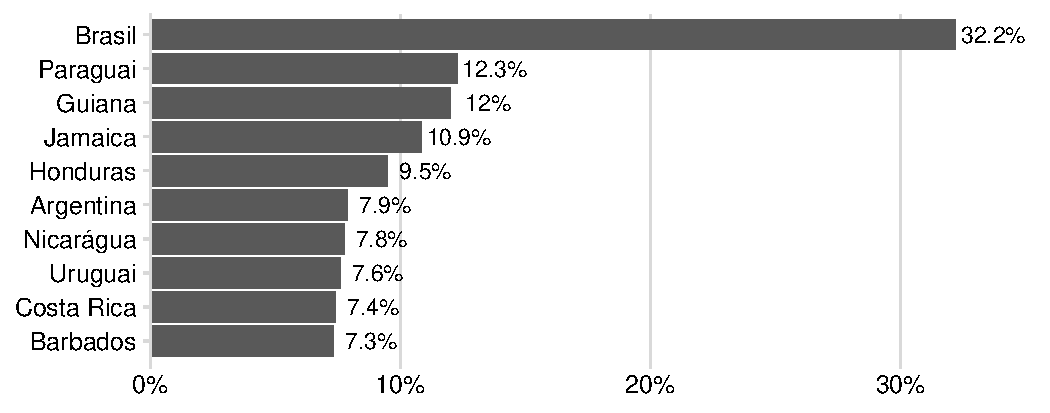
\includegraphics[width = 0.9\textwidth, scale=1]{spread_AL.pdf}
        \legend{Fonte: indicador ``FR.INR.LNDP'' do World Bank. Elaboração própria}
        \label{spreadal}
    \end{figure}

    Com a bem-sucedida estabilização macroeconômica levada a cabo pelo Plano Real, esperava-se que esse nível finalmente começasse a convergir para os padrões internacionais mas, embora ele tenha de fato caído bastante, ainda continuou em um patamar relativamente bastante elevado.

    Desde então, uma das principais razões a que se vem atribuindo a isso é a política monetária, conduzida sob o Regime de Metas de Inflação (RMI) desde 1999, de manter a taxa básica de juros a níveis bastante elevados, com o objetivo de controlar a inflação. O spread, por ser, do ponto de vista ex-ante (ou antes do resultado financeiro das operações do banco), a diferença entre a taxa pela qual o banco empresta e a taxa pela qual ele capta recurso, a taxa básica de juros influencia diretamente o spread por representar um custo de oportunidade para a operação de crédito, visto que a Selic serve como indexador de parte dos títulos da dívida brasileira, uma aplicação muito menos arriscada e mais líquida que o crédito \cite[p.~7]{manhica12}.

    Mais recentemente, o debate foi reanimado devido à persistente queda da taxa Selic, trazendo consigo a expectativa de queda também do spread. Embora essa queda tenha mesmo se efetivado, seu ritmo foi tido como insatisfatório pelas autoridades \cite{valor1}. Há um elenco de fatores que podem ajudar a explicar isso, de variáveis micro, como a concorrência, assimetrias de informação sobre os tomadores de crédito e capacidade de recuperação de garantias\footnote{Ver \cite[p.~13]{reb2018}.}, a macroeconômicas, como a inadimplência e concentração bancária\footnote{Ver \cite{valor2}}.
    
    Em um cenário de incerteza macroeconômica, é interessante que se investigue os determinantes macroeconômicos do spread bancário, a fim de, com um melhor entendimento do caso brasileiro, contribuir para a efetividade das políticas de redução do spread, o que se apresenta ainda mais importante na atual situação de estagnação econômica, já que um spread mais baixo poderia ajudar na retomada, ao facilitar o acesso ao crédito dos agentes econômicos e, portanto, a realização de investimentos \cite[p.~8]{manhica12} além de, de modo geral, significar um sistema financeiro mais desenvolvido, com mais eficiência na intermediação financeira.

\section{Visualização e análise descritiva das variáveis}

    Este capítulo pretende apresentar as relações teóricas entre a variável dependente e as variáveis independentes incluídas no modelo, assim como a evolução histórica das séries, abrangendo o período de março de 2011 a dezembro de 2018.

    Primeiro, o spread bancário. Trata-se, mais especificamente, da série 20786 do Sistema Gerenciador de Séries Temporais (SGS) do Banco Central do Brasil, intitulada "Spread médio das operações de crédito com recursos livres - Total", sendo a diferença, em pontos percentuais, entre a taxa média de empréstimo e de captação no mês. Por total, entende-se que ela aglutina operações de pessoas físicas e jurídicas, e por recursos livres, que exclui operações envolvendo taxas regulamentadas, lastreadas em recursos governamentais e afins.

    Na literatura, é o que se conhece por spread \textit{ex-ante}, porque é calculado antes do resultado, com base nas taxas estabelecidas pelos bancos, decisão em grande parte influenciada por suas expectativas. Por isso, esta taxa é mais volátil e mais sensível a mudanças macroeconômicas e risco percebido \cite[p.~226]{leal07}. Em contraste, o spread \textit{ex-post} é calculado com base na receita e despesa efetiva advinda da atividade de intermediação financeira \cite[p.~2]{almeida15}. 
    
    Na Fig. 1, salta à vista o aumento do spread a partir de 2014, após uma queda que se iniciou por volta de 2012 e que corresponde às políticas do primeiro governo de Dilma Rousseff com o intuito de reduzir o spread via aumento do portfólio de crédito dos bancos públicos, forçando uma queda pela competição das taxas de juros de empréstimos \cite[p.~1]{almeida15}. Porém, com a deterioração das condições macroeconômicas a partir de 2014, observamos a escalada do spread, seguido de um declínio iniciado em 2017 que veio com, entre outras coisas, a queda persistente da taxa SELIC a partir de então.

    \begin{figure}[h]
        \centering
        \caption{Spread médio das operações de crédito com recursos livres - Total}
        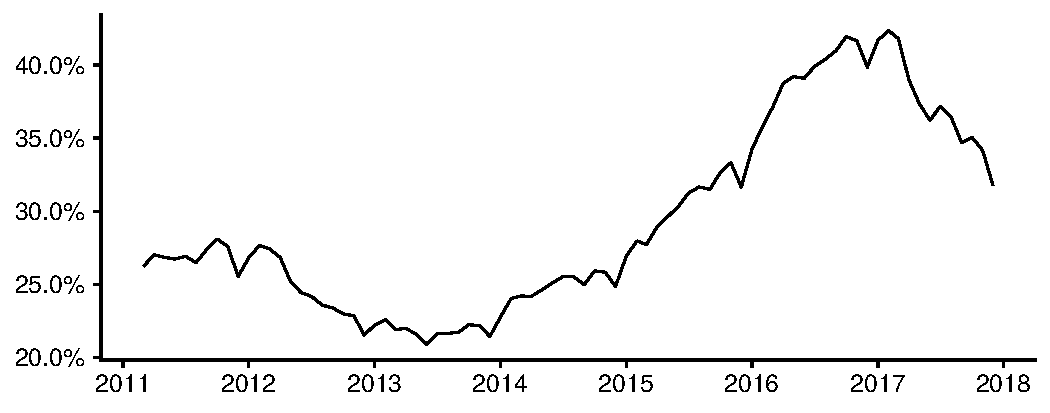
\includegraphics[width = \textwidth, scale=0.75]{Spread.pdf}
        \legend{Fonte: série 20786 do SGS\@. Elaboração própria}
        \label{spread}
    \end{figure}

    Este movimento da taxa SELIC pode ser visto na Fig. 2. A contraposição das duas séries sugere de imediato que elas são positivamente correlacionadas. De fato, é isso o que naturalmente se argumenta, porque uma taxa básica de juros mais elevada implica maior custo de oportunidade para a atividade de crédito, uma vez que aumenta a rentabilidade dos títulos públicos, tornando mais atrativa uma aplicação que já tem a vantagem de ser mais líquida e menos arriscada \cite[p.~372]{oliveira2007}. Por esta razão, é esperado um coeficiente positivo para a taxa básica de juros, pelo efeito custo de oportunidade. Na literatura empírica, não há divergências para essa estimativa, tendo a maior parte dos estudos encontrado a relação esperada \cite[p.~233-234]{leal07}.

    \begin{figure}[h]
        \centering
        \caption{Taxa de juros - Selic acumulada no mês anualizada}
        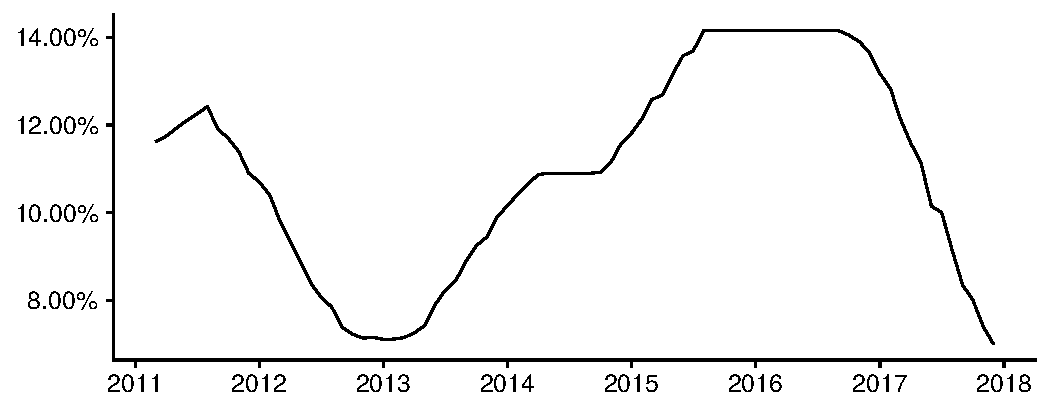
\includegraphics[width = \textwidth, scale=0.75]{Selic.pdf}
        \legend{Fonte: série 4189 do SGS\@. Elaboração própria}
        \label{selic}
    \end{figure}

    Um padrão parecido pode ser observado na série da Inadimplência, na Fig. 3. A inadimplência passou a cair consideravelmente em 2012 para depois aumentar a partir de 2014 e 2015, com o advento da crise econômica. Não é surpreendente que haja uma correlação entre a Selic e a inadimplência, visto que um aumento da taxa básica de juros eleva o custo de captação, que é então repassado para o juros final, prejudicando a capacidade de pagamento \cite[p.~390]{oliveira2007}. A inclusão desta variável, portanto, serve para capturar o efeito do risco de crédito sobre o spread, \textit{ceteris paribus}.

    \begin{figure}[t]
        \centering
        \caption{Inadimplência da carteira de crédito - Total}
        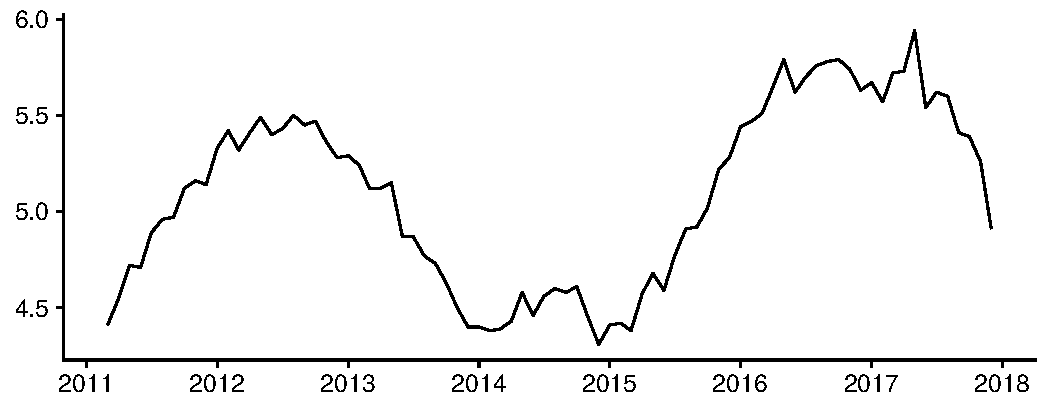
\includegraphics[width = \textwidth, scale=0.75]{Inadimplencia.pdf}
        \legend{Fonte: série 21085 do SGS\@. Elaboração própria}
        \label{inad}
    \end{figure}

    A série de inflação escolhida foi o Índice Geral de Preços (IGP-DI), por ter apresentado resultados mais consistentes que o IPCA \cite[p.~66]{rocha09} e por ser mais abrangente \cite[p.~21]{afanasieff02}. A inclusão dessa variável se faz prudente porque sua variação pode influenciar a taxa básica de juros e a política de juros dos bancos, portanto o spread \cite[p.~14]{bignotto06}. O que se espera obter na estimação é um coeficiente positivo, indicando uma relação direta entre a inflação e o spread, devido ao fato de que em um ambiente econômico não sujeito à instabilidade dos preços os bancos não precisariam se proteger dela via spread. Se por um lado o efeito teórico esperado é claro, o que sairá na estimação é incerto, porque na literatura varia desde insignificante, como em \citeonline{oreiro}, a um sinal inesperado e significante, como em \citeonline{bignotto06} e \citeonline{afanasieff02}\footnote{Como possível causa, os autores indicam a apropriação de receita de senhoriagem com o spread \cite[p.~25]{afanasieff02}}.
    
\begin{figure}[h]
  \centering
    \caption{Índice Geral de Preços (IGP-DI)}
      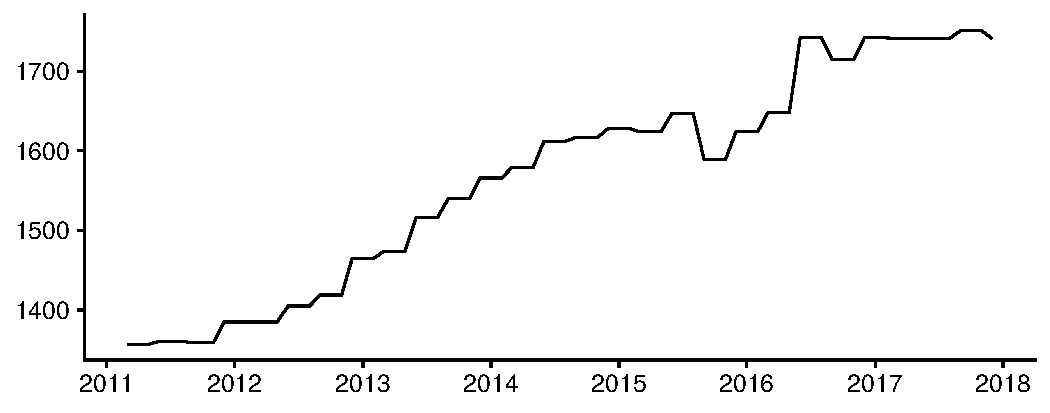
\includegraphics[width = \textwidth, scale=0.75]{IGP.pdf}
      \legend{Fonte: IPEA\@. Elaboração própria}
      \label{igp}
\end{figure}
    
    % TODO: Alterar para Pib Mensal
    A série usada para capturar o efeito da atividade econômica sobre o spread é a Produção da indústria geral, calculada pelo IBGE como a variação percentual em relação ao mesmo período do ano anterior. Segundo \citeonline{oreiro}, o efeito desta variável sobre o spread é incerto, pois duas forças opostas entram em jogo: mais atividade econômica pode resultar em menor spread por reduzir o custo da concessão de crédito via aumento da escala de operação, mas também em maior spread porque mais pessoas demandarão crédito, o que pode elevar as taxas de empréstimo, o que por sua vez depende do poder de mercado dos bancos \citeonline[p.~626]{oreiro}. \citeonline{oreiro} encontram esta última relação na estimação, argumentando ter prevalecido o efeito poder de mercado. Os resultados não tem sido consistentes através dos estudos \cite[p.~236]{leal07}, mas de qualquer forma é considerada adequada sua inclusão como controle, evitando viés de variável omitida.


    \begin{figure}[h]
        \centering
        \caption{Produção da indústria geral}
        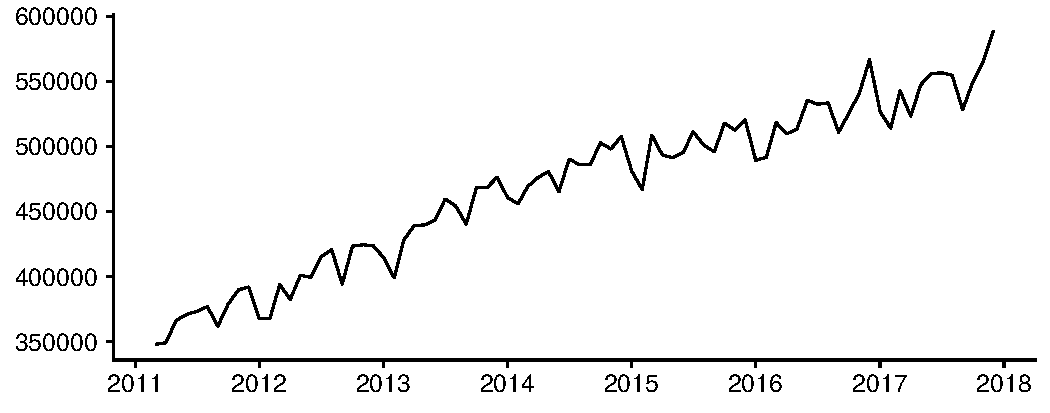
\includegraphics[width = \textwidth, scale=0.75]{PIB_Mensal.pdf}
        \legend{Fonte: IBGE\@. Elaboração própria}
        \label{prodind}
    \end{figure}

    Para a variável de concentração bancária, foi escolhido o índice de Herfindahl-Hirschmann, calculado pelo Banco Central do Brasil e divulgado no Anexo Estatístico do Relatório de Estabilidade Financeira, de abril de 2018. Os dados são trimestrais, por isso a necessidade de extrapolar os valores para os meses adjacentes. Como se sabe, este é um indicador do nível de concentração econômica em um mercado, obtido ao somar o quadrado das participações de cada instituição financeira no mercado considerado, que no nosso caso é o mercado de crédito. O BCB considera um IHH entre 0 e 1000 indicativo de baixa concentração, acima de 1000 e menor que 1800, de moderada concentração e acima de 1800 de alta concentração.

    \begin{figure}[h]
        \centering
        \caption{Índice de Herfindahl-Hirschmann - IHH}
        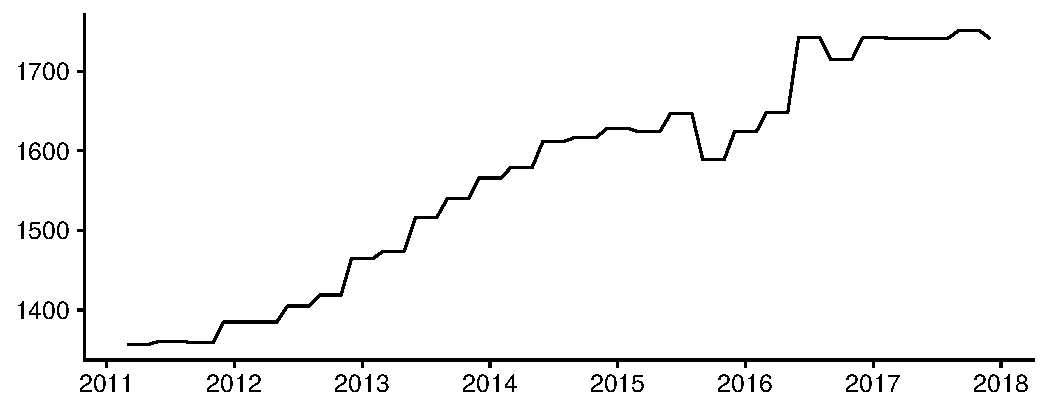
\includegraphics[width = \textwidth, scale=0.75]{IHH.pdf}
        \legend{Fonte: BCB\@. Elaboração própria}
        \label{ihh}
    \end{figure}

    Fica nítida a tendência de ascensão da concentração bancária, só refreada no final de 2015, voltando a crescer em seguida para depois permanecer estagnada, em um nível próximo do que é considerado uma concentração alta.

    No entanto, é preciso cautela na análise da concentração bancária como determinante do spread, já que a literatura sobre o assunto está longe de ser conclusiva \cite[p.~11]{reb2017}. De fato, como explicita \citeonline{reb2017}, há alta concentração bancária mesmo em países com um sistema financeiro considerado desenvolvido, isso porque esta indústria exige ganhos de escala e altos investimentos, o que está ligado à eficiência da intermediação financeira, que ajuda a reduzir o spread. Portanto, é possível que se encontre até mesmo uma relação inversa entre concentração e spread. 

    O relatório explica então que a variável relevante é a concorrência, que cresceu no período de 2000 a 2017 segundo o relatório \cite[p.~11]{reb2017}, ilustrando que maior concentração não implica necessariamente em menor concorrência.

    Dito isto, a inclusão desta variável é justificada pelo interessante aspecto teórico que ela representa. Apesar da dificuldade de predizer o sinal estimado, ainda é razoável que se espere um sinal positivo.

    Por fim, a \autoref{tab1} sumariza o que foi aqui discutido, listando cada variável e seus sinais esperados, além de algumas estatísticas descritivas.

    \begin{table}[h]
        \IBGEtab{\caption{Tabela de estatísticas descritivas}\label{tab1}}
        {%
            \begin{tabular}
                {@{\extracolsep{5pt}}lccccc}
                \midrule
                Variável              & \multicolumn{1}{c}{Média} & \multicolumn{1}{c}{Desvio Padrão} & \multicolumn{1}{c}{Mín.} & \multicolumn{1}{c}{Máx.} & \multicolumn{1}{c}{Sinal esperado} \\
                \midrule
                Spread                & 29,33                     & 6,51                              & 20,89                    & 42,34                    &  \\
                Selic                 & 10,96                     & 2,37                              & 7,00                     & 14,15                    & + \\
                Inadimplência         & 5,09                      & 0,47                              & 4,31                     & 5,94                     & + \\
                IGP-DI                & 5,74                      & 7,33                              & $-$13,93                 & 23,26                    & + \\
                Atividade Econômica   & $-$2,28                   & 4,86                              & $-$13,39                 & 9,70                     & +/- \\
                IHH                   & 1.566,30                  & 133,69                            & 1.357                    & 1.751                    & + \\
                \midrule
            \end{tabular}
        }
        {\fonte{Elaboração própria.}\nota{Em sinal esperado, ``+'' indica um coeficiente positivo, ``-'', um negativo.}}
    \end{table}


\section{Revisão de Literatura}
\subsection{Revisão da literatura teórica}

    Nesta seção pretende-se explorar três modelos que se consagraram na literatura sobre a relação entre spread bancário e concentração bancária: o modelo do banco como uma firma maximizadora de lucros de \citeonline{klein} e o modelo do banco como intermediador financeiro de \citeonline{hoesaunders}. O intuito é explicitar quais variáveis são relevantes para explicar o spread bancário e por quê, de um ponto de vista macro e microeconômico.

\subsubsection{O Banco como firma}

    Neste modelo, o banco é visto como uma firma que produz serviços voltados para intermediar a oferta e demanda de crédito, receber depósitos (D) e fazer empréstimos (L), a uma taxa de juros determinada em um mercado monopolístico ou semi-monopolístico, ou seja, em que tem poder de fixar a taxa de juros acima do custo marginal de produção, e é precisamente nesse sentido que o spread bancário é aqui entendido, como o poder de mercado deste banco. \cite{oreiro}

    O autor considera que o banco seja neutro ao risco, buscando maximizar tão somente o valor esperado do lucro, sem considerar sua variância, deparando-se com uma curva de demanda por empréstimos decrescente, $L(r_L)$, e uma curva de oferta de depósitos crescente, $D(r_D)$, e uma função custo do tipo $C(D, L)$, em que$ r_L$ denota a taxa de juros cobrada ao emprestar, e $r_D$ a paga ao depositante. A função custo, considerando as funções inversas, é assim considerada: \begin{equation}\pi(D, L) = r_L(L)L + rM - r_D(D)D - C(D, L)\end{equation} em que $r$ representa a taxa de juros do mercado interbancário, e M, o que o banco tem disponível para aplicar neste mercado, a saber, tudo o que recebe de depósito e não empresta nem vai para o compulsório (uma taxa $\alpha$), $M = (1 - \alpha)D - L$.

    E assim, manipulando a equação, obtemos o que representa o resultado da intermediação financeira subtraído de seus custos: \begin{equation}\pi(L, D) = (r_L(L) - r)L + (r(1 - \alpha) - r_D(D))D - C(D, L)\end{equation}

    O próximo passo é obter a margem ótima de intermediação, isto é, a que maximiza a função lucro. Para isso, tira-se as derivadas parciais desta função em relação a L e D para se chegar às condições de primeira ordem, e, depois de algumas manipulações algébricas, chega-se às equações fundamentais do modelo:

    \begin{gather}
        \frac{1}{\epsilon^{*}_L} = \frac{r^{*}_L - (r - C^{'}_L)}{r^{*}_L} \\
        \frac{1}{\epsilon^{*}_D} = \frac{r(1-\alpha)-C^{'}_D - r^{*}_D}{r^{*}_D}
    \end{gather}

    O lado direito da equação é a versão para firma bancária do índice de Lerner\footnote{ Definido como a razão $(P - C_{mg}) / P$, em que $P$ é preço e $C_{mg}$ é o custo marginal, é uma medida do poder de mercado de um agente maximizador de lucros, sendo idêntico à recíproca da elasticidade. \cite{maudos}}, sendo, por definição, em cada um dos casos, igual ao inverso da elasticidade-juros da demanda por empréstimos ($\epsilon^{*}_L$) e oferta de depósitos ($\epsilon^{*}_D$). A interpretação desse resultado é que, para maximizar seus lucros, os bancos procuram fixar a taxa de juros num nível acima de seus custos, mas não ao ponto de perderem muitos clientes para a concorrência (o que acontece mais facilmente em mercados com demanda elástica etc.).

    Segue-se imediatamente destas equações que o spread bancário será tão maior quanto menos sensíveis forem as elasticidades da demanda por empréstimo e da oferta de depósito em relação à taxa de juros. Outra implicação interessante, e nada óbvia é de que, se a taxa de juros $r$ do mercado interbancário aumentar, as taxas de intermediação também irão \cite[p.~59]{freixas}.

\subsubsection{O banco como intermediador financeiro}

    Neste modelo, primeiro apresentado em \citeonline{hoesaunders}, o banco é considerado como um agente que atua como intermediador entre demandantes e ofertantes de fundos. É um dos mais influentes modelos na literatura, tendo sido estendido por vários outros autores, das quais se falará mais adiante de \citeonline{maudos}.

    Este modelo difere radicalmente do de \citeonline{klein} no que tange ao tipo de mercado em que o banco atua, não mais harmônico e equilibrado, mas sujeito a incertezas. Neste cenário, o banco não é mais considerado neutro ao risco, mas avesso a ele. Isso porque se depara com duas incertezas: o risco da inadimplência e o risco da taxa de juros, que tem a ver com a possível descoordenação entre demanda por empréstimos e ofertas de depósitos, caso em que o banco terá que recorrer ao mercado interbancário. No caso de demanda excessiva de empréstimos, o banco terá que pedir emprestado e estará sujeito ao risco da taxa de juros aumentar nesse ínterim. No caso de oferta excessiva de depósitos, terá que aplicar o excesso, no que estará sujeito ao risco da taxa cair. \citeonline[p.~2262]{maudos}

    Por esta razão, os bancos procuram minimizar esse risco fixando taxas de juros para os depósitos ($r_D$) e para os empréstimos ($r_L$) com a adição de uma pequena margem relativa à taxa de juros do mercado interbancário. Esta margem é o spread ($s$):

	\begin{align}
        r_D &= r - a \\
        r_L &= r + b \\
        s &= r_L - r_D = a + b
	\end{align}

    Para uma derivação das equações do modelo, até a equação do spread ótimo, ver \citeonline[p.~2262]{maudos} ou \citeonline[p.~584]{hoesaunders}. Para propósitos da revisão, iremos omiti-la, considerando somente suas implicações no que concerne aos determinantes do spread. São eles:

	\begin{enumerate}
		\item Estrutura competitiva do mercado: o que se relaciona com as elasticidades-juros da demanda por empréstimo e da oferta de depósitos, como em \citeonline{klein}.
		\item Aversão ao risco: quanto mais avessos, maior o spread.
		\item Volatilidade da taxa de juros do mercado interbancário: quanto mais instável a taxa de juros, maior o risco, e portanto maior o spread.
		\item Inadimplência: quanto maior o risco de inadimplência, mais o bancos terão que se proteger via spread.
		\item Covariância entre risco da taxa de juros e de inadimplência: captura a influência da instabilidade macroeconômica na insolvência das famílias. \cite{oreiro}
		\item Tamanho médio das operações de crédito e de depósito: uma operação de tamanho maior que o médio significa maior perda potencial, da qual se protege com um spread maior.
	\end{enumerate}

    Esse modelo teórico é a base sob a qual se sustenta a abordagem empírica dos mesmos autores: a estimação do spread em dois estágios. Primeiro, estima-se o spread "puro", usando as variáveis não incluídas no modelo teórico como controle, comumente variáveis microeconômicas e características dos bancos, para então regredi-lo contra as variáveis do modelo teórico \citeonline{maudos}. Como será visto adiante, uma das vantagens dessa abordagem está em sua flexibilidade, permitindo a inclusão de variáveis sem grandes problemas \citeonline[p.~2]{almeida15}.

\subsection{Revisão da literatura empírica}

    Esta seção procura revisar os estudos empíricos sobre os determinantes do spread bancário que, cabe antes esclarecer, é calculado com base nas taxas de juros prefixadas cobradas nas modalidades de crédito com recursos livres e na taxa de captação de CDB de trinta dias.

    A estabilidade macroeconômica e as políticas governamentais que se seguiram ao Plano Real possibilitaram uma queda significativa do spread bancário, porém somente até um nível considerado ainda bastante alto para os padrões internacionais. Somando-se a isso a reestruturação bancária observada no período, \citeonline{afanasieff02} notam que além da grande variação temporal do spread, há também uma grande variação interbancária. É nesse sentido em que os autores justificam o emprego de técnicas de dados em painel, com o objetivo de capturar essas características do mercado bancário brasileiro para a decomposição dos principais determinantes do spread em variáveis micro e macroeconômicas.

    Para isso, os autores aplicam a metodologia de dois passos de \citeonline{hoesaunders}, usando dados mensais de 142 bancos para o período de fevereiro de 1997 a novembro de 2000, formando um painel com 5578 observações. Para a estimação do spread puro, usam como regressores o intercepto, um vetor temporal e um de características bancárias como controle\footnote{Dentre elas, número de agências, custos operacionais, a taxa de depósitos à vista e a prazo em relação ao ativo total, sendo duas variáveis distintas, a liquidez, pagamento de juros implícitos, alavancagem, uma variável dummy para banco estrangeiro, a receita de serviços sobre a receita operacional total e o patrimônio líquido}. Uma vez estimado o spread puro, dado nesse caso pelos coeficientes do vetor temporal e do intercepto, ele é então regredido contra as variáveis macroeconômicas: a taxa de inflação, o compulsório, a taxa SELIC, o crescimento do PIB, a taxação financeira e uma proxy para prêmio de risco.

    No primeiro estágio, foi encontrado que o custo operacional, a taxa de depósitos à vista em relação ao ativo total e a de receita de serviços em relação à receita operacional afetam positivamente o spread, e que os bancos estrangeiros estão em média associados a um spread menor. Os autores, ao contraporem o spread puro estimado com o observado, apontam ainda que os fatores microeconômicos não parecem ser os principais determinantes do spread.
    
    Pelos resultados do segundo estágio, há uma relação direta e significativa entre spread e taxa básica de juros, risco, taxação financeira e crescimento do PIB, e contrária no caso da inflação. O efeito estimado do compulsório não foi significativo. Os autores, por fim, concluem que este é um resultado coerente com a o fenômeno de estabilização macroeconômica da época, mas chamam a atenção para a ineficiência e disparidade no mercado bancário, que tornam possível que bancos atuem cobrando taxas muito maiores que seus rivais.

    Seguindo linha metodológica parecida, \citeonline{bignotto06} também se utilizam do modelo teórico de \citeonline{hoesaunders} para analisar a influência dos custos de intermediação e dos fatores de risco de crédito e de juros sobre o spread. Para a estimação, fez-se uso de dados de 87 bancos brasileiros ao longo do 1º trimestre de 2001 até o 1º trimestre de 2004, formando uma base de dados em painel desbalanceado com 1131 observações.
    
    Foram usados como regressores o custo administrativo, uma proxy para o risco de crédito e de juros, o market-share, o risco de liquidez, a taxa de receitas de serviços sobre o ativo total e a da despesa tributária sobre o ativo total, o compulsório, a SELIC, a inflação e o ativo total de cada banco corrigido pela inflação, além de uma variável não-observável de aversão ao risco como controle. 
    
    O modelo que os autores julgam mais eficiente revela uma relação direta entre o spread e os custos administrativos, o risco de crédito e de juros, o compulsório, a SELIC, e o ativo total, todos com o sinal esperado. Algumas variáveis de controle apresentaram coeficientes inesperados, como no caso da liquidez, da receita de serviços e do market share. Já a variável relativa à carga tributária não se mostrou significativa.

    Complementando os importantes estudos feitos pelo Banco Central do Brasil à época, que consistiam na decomposição contábil do spread, \citeonline{nakane02} buscaram investigar a sensibilidade do spread a variações nas variáveis que o compõem, isto é, investigar o assunto por um abordagem econométrica. Para isso, os autores utilizaram a seguinte equação:

    $$\ln spread = \beta_0Tend + \beta_1\ln selic_t + \beta_2\ln adm_t + \beta_3\ln risk_t + \beta_4\ln imp_t + \beta_4\ln comp_t$$

    Em que $selic$ é a taxa básica de juros, $adm$ é a razão das despesas administrativas sobre o volume de crédito, $risk$ é uma proxy de risco global\footnote{"[É ] o spread do rendimento do C-Bond sobre o rendimento do título do Tesouro americano com mesma maturidade." \cite[p.~10]{nakane02}} que busca capturar expectativas, algo mais apropriado quando se trata do spread ex-ante, $imp$ é uma medida da incidência de tributos indiretos sobre o spread, $comp$ é a taxa de compulsório sobre depósitos à vista exigida pelo Bacen,  $Tend$ é uma medida de tendência determinista incluída com o intuito de controlar para variáveis que não foram incluídas na equação, como a taxa de inflação, o nível de atividade econômica etc. e $\ln$ é o logaritmo natural.  Para mais detalhes, ver \citeonline[p.~10]{nakane02}

    Para a estimação da equação de longo prazo, foram usados dados mensais do período de agosto de 1994 a setembro de 2001 em um modelo de vetores autorregressivos (VAR) que, uma vez tratado estatisticamente, revelou que a taxa Selic, as despesas administrativas, o risco e os impostos indiretos afetam positiva e significativamente o spread. Já o compulsório não se mostrou significativo e foi retirado do modelo.

    Em seguida, os autores decompuseram o spread do período com base nessa estimação. O resultado indica que todas as variáveis são bem relevantes na composição do spread no período, em especial a variável de risco, relevância esta que foi aumentando com o passar dos anos e que é análoga à considerável participação da inadimplência na decomposição contábil do spread. Os custos administrativos e a Selic vêm em seguida em importância, ambas com tendências sutilmente declinantes. E, por fim, a importância relativa dos impostos indiretos é a menos sobressalente, mas aumentou com os anos. 

    Um artigo que segue um caminho semelhante em termos de modelagem é o de \citeonline{oreiro}, já que para a estimação dos determinantes também se utilizou um modelo VAR. Este estudo, porém, se distingue por dar foco aos efeitos das variáveis macroeconômicas sobre o spread, cobrindo o período de janeiro de 1995 a dezembro de 2003. 
    
    São usados como regressores séries de frequência mensal como o nível da taxa básica de juros (SELIC) e sua volatilidade (como proxy para o risco de juros), o nível de atividade econômica, o recolhimento compulsório sobre depósitos à vista e a inflação.

    Para interpretar os coeficientes estimados, os autores se utilizaram da função de impulso-resposta, em que se procurou observar o efeito de longo prazo que um choque exógeno de um desvio-padrão em uma variável independente tem sobre a variável dependente. A decomposição da variância também foi utilizada, com objetivo similar. Em ambos os casos, busca-se enxergar o efeito estimado do choque ao longo de 12 meses.

    Os resultados mostram que um choque exógeno no nível e volatilidade da taxa de juros tem um efeito positivo e persistente sobre o spread, como esperado. Um choque na proxy para o nível de atividade econômica mostrou ter um impacto positivo, o que os autores interpretaram como um possível efeito do poder de mercado dos bancos prevalecendo sobre o efeito inadimplência. O efeito de um choque na inflação se mostrou insignificante estatisticamente. Eles concluem dizendo que um ambiente macroeconômico estável é uma condição indispensável para reduzir o spread.

\section{Referencial Metodológico}

    Neste capítulo serão brevemente apresentadas as metodologias utilizadas para a modelagem e tratamento de séries temporais.

    Todo estudo do tipo requer primeiro que conheçamos a ordem de integração das séries, isto é, se é estacionária (caso em que é integrada de ordem 0) ou, caso contrário, quantas $d$ vezes é preciso diferenciá-la para que se torne estacionária (caso em que será integrada de ordem $d$), o que é mais formalmente feito com um teste de raiz unitária.

    Uma vez que se saiba quais são as séries não-estacionárias, é prudente investigar se alguma combinação linear delas é estacionária, ou seja, se há co-integração.

    Os resultados destes dois testes influenciam enormemente na decisão de como modelar o relacionamento entre as séries. 

    \subsection{Teste de raiz unitária}

    Na análise de séries temporais, é comum nos assegurarmos de que elas sigam um processo estocástico cujas variáveis aleatórias tenham média constante, variância constante e finita e função de autocovariância que dependa somente da defasagem no tempo e não do tempo em si \cite[p.~734]{gujarati}, isto é, que sejam estacionárias no sentido amplo. Mais formalmente, um processo aleatório formado por variáveis aleatórias discretas $Y_t$ será estacionário se:

    Dado um processo estocástico autorregressivo de ordem 1:

    \begin{equation}\label{processo_estocastico} Y_t = \rho Y_{t-1} + u_t \end{equation}

    Onde $ u_t \stackrel{iid}{\sim} \text{N}(0,\text{ }\sigma^2) $. Sabe-se que ele será estacionário se $ \lvert \rho \rvert < 1 $, e não-estacionário se $ \lvert \rho \rvert = 1 $, o que é conhecido como passeio aleatório\footnote{Ao resolver recursivamente para o caso quando $ \lvert \rho \rvert = 1 $, $ Y_t = Y_{t-1} + u_t = Y_0 + \sum u_t $, pode-se perceber a importante característica da memória infinita, de que ele nunca se esquece do choque, o que também se conhece por tendência estocástica \cite[p.~736]{gujarati}}.

    O objetivo do teste de raiz unitária é inferir o valor de $ \rho $ com base nas realizações particulares do processo estocástico. O teste Augmented Dickey-Fuller o faz ao modificar \eqref{processo_estocastico} como segue:

    \begin{align}
        \label{adf}
        Y_t - Y_{t-1} &= \rho Y_{t-1} - Y_{t-1} + \sum_{i = 1}^{p-1}\delta \Delta Y_{t-i} + u_t \nonumber \\
        \Delta Y_t &= \gamma Y_{t-1} + \sum_{i = 1}^{p-1}\delta \Delta Y_{t-i} + u_t
    \end{align}

    Onde $ \gamma = (\rho - 1) $. Para logo depois estimar esta equação por Mínimos Quadrados Ordinários (MQO).
   
    O valor estimado de $ \gamma $ serve então para testar a hipótese de raiz unitária $ \gamma = 0 $, que equivale a $ \rho = 1 $, contra a hipótese alternativa unilateral $ \gamma < 0 $, que equivale a $ \rho < 1 $. Calcula-se então o valor t estimado, isto é, $ \hat{\gamma} / \text{EP}(\hat{\gamma}) $, com o porém de que sob a hipótese nula $ \gamma = 0 $, essa estatística não segue mais a distribuição t, mas a distribuição $ \tau $. Isso se dá em razão do teste t ser enviesado no caso de um passeio aleatório \cite[p.~748-749]{gujarati}.

    Importante pontuar que a estatística $ \tau $ é sensível à forma funcional da equação \eqref{processo_estocastico}, isso quer dizer que os valores críticos do teste mudarão se adicionarmos um termo de deslocamento $ \delta $ em \eqref{processo_estocastico}, que denotaremos por $ \tau_{\mu} $ ou um termo de tendência determinística, $ \beta t $, $ \tau_{\tau} $.
   
    O termo adicional $ \sum_{i = 1}^{p-1}\delta \Delta Y_{t-i} $ em \eqref{adf} serve para generalizar o teste para processos autorregressivos de ordem $ p $, de forma a preservar a condição de ruído branco em $ u_t $ \cite[p.~40]{gustavo}.

    Uma série é dita integrada de ordem 0 quando for diagnosticada como estacionária, $ Y_t \sim I(0) $, e integrada de ordem $ d $ quando é necessário diferenciá-la $ d $ vezes para torná-la estacionária, $ Y_t \sim I(d) $ \cite[p.~740]{gujarati}.

    \subsection{Teste de Co-integração}

    Quando duas ou mais séries são integradas da mesma ordem, mas uma combinação linear delas for integrada de uma ordem menor, dizemos que elas co-integram. O caso comum é quando as séries são não-estacionárias, mas uma combinação linear delas é estacionária. Intuitivamente, isso quer dizer que, apesar da tendência estocástica torná-las imprevisíveis individualmente, há um mecanismo de equilíbrio de longo prazo que as impede de se afastarem muito uma da outra (um mecanismo de "correção de erros") \cite[p.~46]{gustavo}.

    Formalmente, as séries $ \mathbf{Y_t} $ são co-integradas de ardem $ d, b $ se todas forem integradas de ordem $ d $ e se existe uma combinação linear $ \mathbf{Z_t} = \pmb{\beta}'\mathbf{Y_t} $ tal que $ \mathbf{Z_t} \sim I(d - b), b > 0 $ \cite[p.~245]{lutkepool}, onde $ \pmb{\beta} $ é um vetor cointegrante.

    O teste de Engle-Granger procura testar essa condição em duas etapas. Em um contexto bi-variado, em que $ Y_t $ é explicada por $ X_t $, estima-se a equação por MQO:

    $$  Y_t = \beta_0 + \beta_1 X_t + u_t \label{engle-granger}$$

    Para na segunda etapa, aplicar o teste ADF nos resíduos desta regressão, ou seja, na equação $ \Delta \hat{u}_t = \gamma \hat{u}_{t-1} + \epsilon_{t} $. Se eles forem estacionários, então pode-se concluir que as séries são co-integradas. Vale ressaltar que, como explicado por \citeonline[p.~756]{gujarati}, os valores críticos com os quais se deve comparar a estatística de teste calculada são diferentes dos do teste de raiz unitária, porque os resíduos a serem testados foram obtidos com base no $ \beta $ estimado.

    Como a relação de co-integração é inerentemente multivariada, este teste não suporta muito bem este caso já que se baseia nos resultados da regressão uniequacional. Além disso, ele depende de como se especifica esta equação, qual variável é endógena e quais são exógenas. Por isso, é apropriado que se investigue a co-integração no contexto multivariado, o que é feito pelo procedimento de Johansen, como veremos \cite[p.~3]{coint2}.

    \subsection{Vetores autorregressivos (VAR)}

    Segundo Grôppo (2004, p. 51-52), a principal característica de um modelo VAR é o tratamento simétrico das variáveis incluídas no modelo, isto é, não é preciso especificar previamente quais variáveis são exógenas e endógenas, o modelo estrutural que espelha o relacionamento real das variáveis. Por isso, ele está sujeito a poucas restrições teóricas. É somente necessário especificar quais variáveis interagem dentro do sistema e o número de defasagens a serem incluída de forma a melhor capturar esta interação.
    
    São muito úteis para visualizar como uma variável responde a um choque em outra variável, através das funções de impulso-resposta. 

    Seguindo a notação de \citeonline[p.~13]{lutkepool}, um modelo de vetores autorregressivos de ordem p, VAR(p), com K variáveis, possui a seguinte forma:

    \begin{equation}
        \label{VAR}
        y_t = v + A_1 y_{t-1} + \dots + A_p y_{t-p} + u_t,\text{\ \ } t = 0, \pm 1, \pm 2, \dots
    \end{equation}

    Onde $ y_t = (y_{1t}, \cdots, y_{Kt})^{'} $ é um vetor de variáveis aleatórias, $ v  = (v_{1}, \cdots, v_{K})^{'}  $, um vetor para o intercepto, $ u = (u_{1}, \cdots, u_{K})^{'} $, um vetor de ruído branco gaussiano\footnote{Logo, $ \mathbb{E}(u_t) = 0 $ e $ \mathbb{E}(u_t u^{'}_t) = \Sigma_{u} $, onde $ \mathbb{E}(u_tu^{'}_s) = 0 $ para $ t \neq s $ e $ \mathbb{E}(u_t u^{'}_t) = \Sigma_u, \forall t $.} e $ A_i $ são matrizes $ (K \times K) $ de coeficientes.

    Desta equação pode-se perceber que os valores presentes das variáveis são explicados pelas $ p $ defasagens de todas as outras variáveis no sistema.

    Dado um AR(1) que começa em $ t = 1 $, resolvendo recursivamente o sistema, chegamos a:

    \begin{align}
        \label{VAR1}
        y_1 &= v + A_1 y_0 + u_1 \nonumber \\
        y_2 &= v + A_2 y_1 + u_2 = v + A_1(v + A_1y_0 + u_1) + u_2 \nonumber  \\
            &= (I_K + A_1)v + A^{2}_1 y_0 + A_1 u_t + u_t \nonumber \\
        y_t &= (I_K + A_1 + \dots + A^{t-1}_1)v + A^{t}_1 y_0 + \sum^{t-1}_{i=0} A^{i}_1 u_t
    \end{align}

    Se todos os autovalores em módulo da matriz $ A_1 $ são menores que 1, o que é equivalente a testar se $ det(I_{K} - A_1z) \neq 0 $ para $ \lvert z \rvert \leq 1 $, o VAR é dito estável e converge assintoticamente para

    \begin{equation}
        \label{ma}
        \begin{aligned}
        y_t &= (I_K - A_1)^{-1} v + \sum^{\infty}_{i=0} A^{i}_1 u_{t-1} \nonumber \\
        y_t &= \mu + \sum^{\infty}_{i=0} A^{i}_1 u_{t-1}
        \end{aligned}
    \end{equation}

    O que é também conhecido como a representação em média móvel do modelo VAR. Dela podemos ver que a distribuição de probabilidades de $ y_t $ é unicamente determinada pela distribuição do termo de erro $ u_t $, que se assume ser gaussiano. Esse resultado pode ser generalizado para AR(p), dado que qualquer processo AR(p) pode ser representado como um processo AR(1) \cite[p.~15]{lutkepool}. Da equação \eqref{ma} a média e auto-covariâncias de $ y_t $ podem ser derivadas: 

    \begin{align*}
        \label{momentos}
        \mathbb{E}(y_t) &= \mu, \forall t \\
        \Gamma_y (h) &= \mathbb{E}(y_t - \mu)(y_{t-h} - \mu)^{'} = \sum_{i=0}^{\infty}A_1^{h+i}\Sigma_uA_1^{i}^{'}
    \end{align*}

    Do que se conclui que um modelo AR(p) estável é estacionário no sentido amplo \cite[p.~15-16]{lutkepool}

    \subsection{Função de Impulso-resposta}

    A função de impulso-resposta serve para visualizar o efeito provocado por um choque exógeno em uma variável em um sistema dinâmico de equações.

    Para vermos o que ocorre matematicamente, seguimos a exposição de \citeonline[p.~51-53]{lutkepool} e supomos um AR(1) com $ v = 0 $, ou seja, $ y_t = A_1 y_{t-1} + u_t $:

    \begin{equation*}
        \label{impulse-response}
        \begin{bmatrix}
            y_{1,t} \\
            y_{2,t} \\
            y_{3,t}
        \end{bmatrix} =
        A_1
        % \begin{bmatrix}
        %     a_{1,1} & a_{1,2} & a_{1,3} \\
        %     a_{2,1} & a_{2,2} & a_{2,3} \\
        %     a_{3,1} & a_{3,2} & a_{3,3} \\
        % \end{bmatrix}
        \begin{bmatrix}
            y_{1,t-1} \\
            y_{2,t-1} \\
            y_{3,t-1}
        \end{bmatrix} +
        \begin{bmatrix}
            u_{1,t} \\
            u_{2,t} \\
            u_{3,t}
        \end{bmatrix}
    \end{equation*}

    Se assumirmos que no período $ t = 0 $ há um choque exógeno em $ y_1 $, tal que

    \begin{equation*}
        \label{impulse-response}
        \begin{bmatrix}
            y_{1,0} \\
            y_{2,0} \\
            y_{3,0}
        \end{bmatrix} =
        \begin{bmatrix}
            u_{1,0} \\
            u_{2,0} \\
            u_{3,0}
        \end{bmatrix} =
        \begin{bmatrix}
            1 \\
            0 \\
            0
        \end{bmatrix}
    \end{equation*}

    Teremos, em $ t $ períodos a frente que

    \begin{equation*}
        \label{impulse-response}
        \begin{bmatrix}
            y_{1,t} \\
            y_{2,t} \\
            y_{3,t}
        \end{bmatrix} =
        A_1^{t}
        \begin{bmatrix}
            1 \\
            0 \\
            0
        \end{bmatrix}
    \end{equation*}

    Do que se conclui que a resposta do sistema a um impulso na variável $ y_1 $ é simplesmente a primeira coluna da matriz $ A_1^{t} $, ou, mais geralmente, a resposta a um impulso na variável $ y_k $, após $ t $ períodos, é a coluna $ k $ da matriz $ A_k^{t} $, que, deve-se observar, vai se aproximando de zero quando $ i $ tende ao infinito se o VAR(1) é estável, ou seja, a resposta do sistema vai se dissipando com o tempo.

   Quando duas variáveis distintas são correlacionadas no sistema, recomenda-se que se visualize a função de resposta ao impulso ortogonal, porque neste caso um choque não pode ser assumido independente um do outro, sendo provável que afete outra variável no período $ 0 $.

    \subsection{Modelo de correção de erros}

    Se há alguma relação de equilíbrio entre as variáveis sob análise, gostaríamos de identificá-la, o que normalmente se faz por um teste. Como observado antes, o teste de co-integração uniequacional não é o mais recomendado para um modelo multivariado.
    
    Nesta seção será introduzido o procedimento de Johansen para identificar relações de co-integração em um sistema de equação, mas antes será preciso apresentar o que é o modelo de correção de erros e sua representação em VAR.

    Em um modelo de correção de erros, a variação das variáveis depende dos desvios em relação ao equilíbrio entre as variáveis (ao desequilíbrio) e de suas variações defasadas. Por exemplo, dadas duas variáveis $ I(1) $, $ y_1 $ e $ y_2 $, teremos que:

    \begin{equation}
        \begin{aligned}
            \label{ecm}
            \Delta y_{1t} = \alpha_1 (y_{1,t-1} - \beta_1 y_{2, t-1}) + \gamma_{11,1} \Delta y_{1,t-1} + \gamma_{12,1} \Delta y_{2,t-1} + u_{1t} \\
            \Delta y_{2t} = \alpha_2 (y_{1,t-1} - \beta_1 y_{2, t-1}) + \gamma_{21,1} \Delta y_{1,t-1} + \gamma_{22,1} \Delta y_{2,t-1} + u_{2t}
        \end{aligned}
    \end{equation}

    Por serem $ I(1) $, as primeiras diferenças $ \Delta y_{i,t} $ são estacionárias e o termo de erro $ u_{it} $ é também assumido estacionário. Colocando o termo de equilíbrio em evidência:

    \begin{align*}
        \alpha_i (y_{1,t-1} - \beta_1 y_{2, t-1}) = \Delta y_{it} - \gamma_{i1,1} \Delta y_{1,t-1} - \gamma_{i2,1} \Delta y_{2,t-1} - u_{it}
    \end{align*}

    Podemos concluir que se algum $ \alpha_{it} \neq 0 $, $ y_{1t} - \beta y_{2t} $ é estacionária, as duas variáveis co-integram, visto que um processo estacionário não pode ser igual a um processo não-estacionário \cite[p.~244-247]{lutkepool}.

    Em notação matricial, as equações \eqref{ecm} tornam-se:

    \begin{equation}
        \label{vecm}
        \begin{aligned}
            \Delta y_t &= \alpha \beta^{'} y_{t-1} + \Gamma_1(y_{t-1} - y_{t-2}) + u_t \\
            y_t - y_{t-1} &= \alpha \beta^{'} y_{t-1} + \Gamma_1(y_{t-1} - y_{t-2}) + u_t \\
        \end{aligned}
    \end{equation}

    O que pode ser representado por um VAR(2) ao manipular algebricamente \eqref{vecm}:

    \begin{equation}
        \label{vecm-var}
        y_t = (I_K + \Gamma_1 + \alpha \beta^{'})y_{t-1} - \Gamma_1 y_{t-2} + u_t
    \end{equation}

    Mais geralmente, supondo um processo VAR(p) instável:
    
    \begin{equation}
        \label{varp_example}
        y_t = A_1 y_{t-1} + A_2 y_{t-1} + \dots + A_p y_{t-1} + u_t 
    \end{equation}

    O que é verdadeiro se $ det(I_K - A_1z - A_2z^2 - \dots - A_pz^p) = 0 $ para $ z = 1 $. Neste caso, conclui-se que a matriz $ \Pi = -(I_K - A_1 - A_2 - \dots - A_p) $ não é inversível e, por isso, $ \text{posto}(\Pi) = r < K $.
    
    Assim, é possível decompôr a matriz $ \Pi $ em duas matrizes \alpha $ e $ \beta $, de posto $ r $ e dimensão $ (K \times r) $ de maneira que $ \Pi = \alpha \beta^{'} $.

   Podemos manipular a equação \eqref{varp_example} tirando a primeira diferença (subtraindo $ y_{t-1} $ de ambos os lados) e manipulando algebricamente de modo a obter a matriz $ \Pi = -(I_K - A_1 - \dots - A_p) $ até chegarmos à representação vetorial de correção de erros:

   \begin{equation}
       \label{vecm_coint}
       \begin{aligned}
           \Delta y_t &= \Pi y_{t-1} + \Gamma_1 \Delta y_{t-1} + \dots + \Gamma_{t-1} \Delta y_{t-p+1} + u_t \\
           \Delta y_t &= \alpha \beta^{'} + \Gamma_1 \Delta y_{t-1} + \dots + \Gamma_{t-1} \Delta y_{t-p+1} + u_t
       \end{aligned}
   \end{equation}

   Onde $ \Gamma_i = -(A_{i+1} + \dots + A_p), i = 1, \dots, p-1 $. É possível ainda reescrever \eqref{vecm_coint} em sua forma VAR, o que não será aqui demonstrado, ver \cite[p.~248-249]{lutkepool}.

   Agora, ao colocar a matriz $ \Pi $ em evidência na equação \eqref{vecm_coint}:

   \begin{equation}
       \label{vecm_coint2}
       \begin{aligned}
       \Pi y_{t-1} = \Delta y_t - \Gamma_1 \Delta y_{t-1} - \dots - \Gamma_{p-1} \Delta y_{t-p+1} - u_t \\
           \alpha \beta^{'} y_{t-1} = \Delta y_t - \Gamma_1 \Delta y_{t-1} - \dots - \Gamma_{p-1} \Delta y_{t-p+1} - u_t
       \end{aligned}
   \end{equation}

   Salta à vista que, se todas as variáveis forem estacionárias após a primeira diferença, ou seja, se são $ I(0) $ ou $ I(1) $, todos os termos do lado direito da equação são estacionários, logo a matriz $ \Pi y_{t-1} = \alpha \beta^{'} y_{t-1} $ também o é. Isto não muda se retirarmos o termo $ \alpha $ do lado esquerdo ao pre-multiplicar a equação por $ (\alpha^{'}\alpha)^{-1}\alpha{'} $, o que nos deixa com $ \beta^{'}y_{t} $, que representa uma relação de co-integração entre as variáveis em $ y_t $. $ \beta $ é conhecida como a matriz de co-integração e $ \alpha $ como a \textit{loading matrix} \cite[p.~244-249]{lutkepool}.

   Quando $ 0 < posto(\Pi) = r < K $, quer dizer que há $ r $ relações de co-integração no sistema. Já quando $ posto(\Pi) = 0 $, ou seja, é uma matriz nula, $ \Delta y_t $ é um VAR(p-1) estável, e se $ posto(\Pi) = K $, quer dizer que todas as variáveis no sistema são estacionárias e que $ \Delta y_t $ pode ser representado por um VAR(p) estável\footnote{Isto se justifica porque, neste caso, $ \Pi = (I_K - A_1 - \dots - A_p) = (I_K - A_1z - \dots - A_pz^p) $ para $ z = 1 $, e, como $ det(I_K - A_1 - \dots - A_p) \neq 0 $, concluímos que o polinômio característico deste VAR não possui raiz unitária, sendo, portanto, estacionário.}.

   \subsection{Teste de Johansen}

   O teste de Johansen, mais detalhadamente explicado em \citeonline[p.~327-330]{lutkepool}, procura testar hipóteses acerca do posto da matriz $ \Pi $ com base numa estatística de teste calculada pela razão entre estimadores de máxima verossimilhança.

   O teste tem duas formas. A primeira calcula uma estatística de teste conhecida como estatística de traço e testa as hipóteses:

   \begin{equation}
       \label{trace}
       \begin{aligned}
           H_0&: posto(\Pi) = r_0 \\
           H_1&: r_0 < posto(\Pi) \leq K
       \end{aligned}
   \end{equation}

   A segunda é conhecida como estatística do máximo autovalor e testa as hipóteses:

   \begin{equation}
       \label{trace}
       \begin{aligned}
           H_0&: posto(\Pi) = r_0 \\
           H_1&: posto(\Pi) = r_0 + 1
       \end{aligned}
   \end{equation}

   Com isso, testam-se as hipóteses nulas de $ posto(\Pi) = r_0 = 0, 1, \dots, K-1 $, até que não se consiga rejeitar a hipótese nula, do que se conclui que o sistema tem $ r_0 $ relações de co-integração.

    % \begin{table}[ht]
    %     \IBGEtab{\caption{Testes de raiz unitária}\label{raiz_unitaria}}
    %     {
    %         \begin{tabular}{lccccccccc}
    %             \midrule
    %             \multicolumn{1}{c}{Variável} & \multicolumn{2}{c}{Sem drift e sem tendência} & \multicolumn{2}{c}{Com drift} & \multicolumn{2}{c}{Com tendência} \\
    %                                 & \tau_1 & 5\%       & \tau_2 & 5\%   & \tau_3 & 5\%     \\
    %             \midrule
    %             spread              & 0.37   & -1.95     & -0.76  & -2.89 & -1.39  & -3.45   \\
    %             selic               & -0.93  & -1.95     & -1.12  & -2.89 & -0.80  & -3.45   \\
    %             pib\_mensal         & 2.15   & -1.95     & -1.43  & -2.89 & -4.23  & -3.45   \\
    %             inad                & 0.23   & -1.95     & -1.45  & -2.89 & -1.12  & -3.45   \\
    %             igp                 & -3.16  & -1.95     & -4.50  & -2.89 & -4.49  & -3.45   \\
    %             ihh                 & 2.56   & -1.95     & -0.93  & -2.89 & -2.25  & -3.45   \\
    %             \midrule
    %         \end{tabular}
    %     } 
    %     {\fonte{Elaboração própria.}}
    % \end{table}

\newpage
\bibliography{../bibliografia}

\end{document}
